\documentclass[../dejiny-rodu-prusiku.tex]{subfiles}

\begin{document}

% str 125 @ 145
\section{Odnož Kostelec nad Mží — větve Výrov}

Potomci Veroniky Prusíkové z Výrova, provdané Hořejšové, podruhé Folkové.

1826 - 1865

Posledním osmým dítětem Vojtěcha Prusíka, výrovského rychtáře, byla dcera Veronika. Narodila se "u Boudů“ na rychtě ve Výrově č. 18 dne 20. 1. 1826. Když jí bylo patnáct let zemřel jí otec. Ve svých dvaceti letech se provdala do vesnice poměrně dosti vzdálené od Výrova. Byl to Kostelec nad Mží a tedy do svého nového domova musela až přes řeku Mži. Veronika vzala si v den svých narozenin 20. 1. 1846 rolníka Jana Horejše. Měla s ním jen dceru Josefu, brzy potom ovdověla. V roce 1854 si vza­la Jana Folka, rodáka z Chotiné, který se do Kostelce nad Mží přiženil. Měli spolu dva syny, Jana a Josefa Folka. Dcera Veroniky z prvního manželství Josefa Horej­šová narodila se 17. 2. 1851 a provdala se za rolníka Výšku v Nadrybech. Tam zemřela 16. 2. 1936. Z druhého man­želství Veroniky roz. Prusíkové ve Výrově, narodil se jí v Kostelci první syn Jan Folk, 4. 6. 1856. Zemřel tam 2. 11. 1936. Druhý syn Josef Folk nar. 18. 3. 1862 přiženil se do Bušovic u Rokycan, kde zemřel 27. 2. 1927. Kostelec nad Mží je hezká, ale opravdu velmi malá vesnice. Má sotva padesát obyvatel. Farností patří k obci Plané, tam se také po smrti všichni obyvatelé Kostelce nad Mží na hřbitově sejdou. Veronika, rodačka výrovská, nebyla dlou­ho v Kostelci, neboť zemřela již 7. 11. 1865 a nebylo jí tedy ani 40 let. To bylo snad příčinou, že styk s tou­to rodovou odnoží býval poměrně malý, později téměř žádný a teprve nyní obnovila se zase všechna spojení příbuzenská a navázaly se přátelské rodové vztahy.

První dítě Veroniky Horejšové roz. Prusíkové byla dcera Josefa. Byla však také jediná z tohoto manželství, poně­vadž Jan Horejš brzy zemřel. Narodila se 17. 2. 1851 a provdala se za rolníka J. Výšku do Nadryb č. 11. V této obci nyní žije mnoho členů našeho rodu. Josefa Výšková měla jediného syna Josefa. Zemřela v Nadrybech 16. 2. 1936.

Syn Josefy Výškové Josef narodil se 24. 3. 1874. Je mu přes 94 let a je dnes nejstarším členem našeho rodu po meči a po přeslici. V době, kdy toto píšeme, je zdráv a čilý. Josef Výška měl čtyři děti. Syny Josefa, Jaromíra, Václava a dceru Annu. Těsně před uzávěrkou zemřel Josef Výška 24. 6. 1968. Nejstarší dítě Josefa Výšky z Nadryb je syn Josef. Narodil se 7. 8. 1901, zůstal na rodném statku v č. 11 a zemřel 30. 12. 1966. Měl jediného syna. Je t0 Vlastislav Výška, nar. 18. 12. 1928 a je agronomem v tamním JZD. U něho bydlí jeho děd Josef, senior našeho rodu. Vlastislav Výška má tři děti. Dcera Milena je narozena 8. 3. 1953, druhá dcera Vlastislava 3. 4. 1954 a syn Jiří Výška nar. 6. 12. 1955.

Druhý syn Josefa Výšky je Jaromír, nar. 23. 7. 1904 a žije v Nadrybech č. 46, kde je členem JZD. Jaromír Výška má jedinou dceru Annu, nar. 3. 4. 1942. Je provdaná Lojdová a má dcerku Ivanu nar. 7. 5. 1967. Bydlí v Kladrubech u Stříbra, Gottwaldova 238.

% str 126 @ 146
Třetím dítětem Josefa Výšky v Nadrybech je dcera Anna. Narodila se 1. 6. 1909, je provdaná Horejšová a bydlí v Nadrybech č. 8. Je bezdětná.

Posledním dítětem Josefa Výšky je syn Václav. Narodil se 10. 3. 1911 v Nadrybech a žije v Kostelci nad Mží č. 2. Tam je členem JZD. Má Jedinou dceru Annu, provdanou Malátovou. Narodila se 6. 1. 1942. Má dcerku Jitku, nar.14. 3. 1963 a bydlí v Týnci u Klatov. Václav Výška v Kostel­ci má ještě syna Václava nar. 27. 3. 1938. Je úředníkem Škodovky a přiženil se do Trnové č. 188.

Když zemřel první manžel Veroniky roz. Prusíkové, Jan Horejš ve svých 33 letech, přiženil se na její usedlost v Kostelci nad Mží č. 7 v roce 1854, Jan Folk z Chotiné. Hospodářství mělo asi 25 ha polí, luk a lesů. Prvním synem Veroniky Folkové byl syn František. Pak následovali ještě Antonín, Bohumil, Václav, Josef a Jan Folkové a dcery Marie a Josefa. Bylo to tedy osm dětí.

Nejstarší František Folk narodil se 29. 1. 1885. Přiženil se do Nadryb, kde měl hospodářství. Zemřel tam 12. 7. 1962. Měl jediné dítě, syna Miloše Folka. Ten se narodil 18. 8. 1922 v Nadrybech. Je automechanikem a v této své činnosti zajíždí často do ciziny. Bydlí v Senci u Zruče na Plzeňsku. Manželkou jeho je také člen našeho rodu, potomek Anny Štěpánkové, roz. Prusíkové z Výrova. Miloš Folk má dvě děti. Syn Miloš narodil se 18. 11. 1949 a Jiří 28. 5. 1951.

Druhé dítě Jana Folka byl syn Antonín. Narodil se 7. 3. 1887 v Kostelci a zde pak převzal po otci hospodářství. Má tři děti. Jeho syn Vratislav Folk nar. 30. 11. 1916 je zemědělským expertem na ONV v Chebu. Tam bydlí ve Šlikově ulici­ č. 12. Měl jedinou dceru Věru nar. 5. 1. 1944. Je učitelkou. Nyní, jako provdaná Trojková bydlí v Kladně, sídliště 9. okrsek, Blok 205/2268.  Druhým dítětem Antonína Folka z Kostelce je dcera Anna. Narodila se 23. 2. 1921 a je provdaná Staňková. Její muž je projektantem podniku Kancelářské stroje. Bydlí v Praze - Malešicích, Tuchorazská 423. Má dvě děti. Dcera Jarmila Staňková je narozena 25. 5. 1947 a syn Milan je narozen 16. 3. 1952. Druhá dcera Antonína Folka je Slávka. Narodila se 18. 5. 1922 a je provdaná Šedivcová v Chrástu u Plzně č. 31. Její syn Vojtěch Še­divec, nar. 1. 11. 1946 bydlí ve Zruči-Senci č. 233. Dcera Miloslava dnes provdaná Kaňková narodila se 18. 9. 1944, bydlí s rodiči v Chrástu č .31. Věra Trojková má syna Josefa nar. 15. 9. 1968.

Třetím dítětem Jana Folka z Kostelce, byla dcera Marie. Narodila se 6. 8. 1889, provdala se za kováře Janovského v Kostelci, ale záhy zemřela. Bylo ji 36 let, když 22. 5. 1925 ukončila svůj život. Měla čtyři děti. Nejstarší byla Anna, nar. 26. 7. 1908 a je dnes provdaná Svejkovská v Týčku č. 26 u Zbiroha. Má dvě děti. Jiří Svejkovský je narozen 5. 2. 1949 a Květa Svejkovská nar. 13. 11. 1943.

% str 127 @ 147
Druhou. dcerou Marie Folkové provdané Janovské je dcera Marie. Narodila se 5. 12. 1909 v Kostelci a bydlí dnes v Plzni Bukovci, Horova 5. Protože se jméno jejího muže Antoušek nelíbilo, převzal p0 svatbě on jméno své ženy. Má dvě děti. Syn Stanislav Janovský nar. 6. 8. 1934 bydlí v Plzni-Slovanech, Bla­tenská 12. Má dceru Janu nar. 29. 7. 1959 a syna Stanislava nar. 5. 10. 1962. Druhé dítě Marie Janovské je Vlasta provdaná Schinabková nar. 3. 9. 1944 a bydlí v Plzni, s rodiči. Třetí dítě Marie Janovské  v Kostel­ci byl syn Jaroslav. Narodil se tam 12. 6. 1912, usadil se v Suchomastech č. 71 u Berouna. Zemřel tam již ve svých 36 letech dne 7. 2. 1952. Zanechal zde dvě děti. Syna Jaroslava nar. 23. 1. 1946 a dceru parcelu Marcelu Janovskou nar. 12. 9. 1951.

Posledním dítětem Marie Janovské roz. Folkové byl syn Václav Janovský. Narodil se 12. 11. 1914 v Kostelci nad Mží, po druhé světové válce usadil se v Záluží u Mostu, ale zde přišel tragicky o život 15. 5. 1948. Jediná jeho dcera Miroslava nar. 4. 7. 1943 je učitel­kou, je provdaná Svobodová a bydlí v Mostě, ul. Vít. Nezvala blok 220-46. Má dcerku Renatu Svobodovou nar. 16. 9. 1967.

Další dcerou Jana Folka byla dcera Josefa. Narodila se 23. 10. 1891 a je provdaná Kroftová v Plzni-Letné, Dlouhá 29. Její dcera Jarmila nar. 23. 9. 1922 je provdaná za podplukovníka Mužíka a bydlí v Chebu, Roose­veltova 28. Má dceru Jarmilu nar. 20. 10. 1944 a Hanu nar. 16. 10. 1946. Druhé dítě Josefy Kroftové je syn Václav. Je narozen 26. 2. 1925 a pracuje ve Škodovce v Plzni. Věra má synka Petra nar. 8. ledna 1968 (Hrdinová). Pátým dítětem Jana Folka byl syn Bohumil. Narodil se v Kostelci 4. 2. 1894 a byl mnoho let zaměstnán v justiční službě v Plzni a v Rokycanech. Z první světové vál­ky se vrátil jako italský legionář. Kratší dobu také byl na frontě francouzské. Bydlí v Plzni, tř. 1. máje č. 2. Bohumil Folk má snad ze všech svých sourozenců nejlepší přehled o své rozvětvené rodině a tato jeho vlastnost dopomáhala také vydatně při pátrání po potomcích Veroni­ky Prusíkcvé, provdané Folkové v Kostelci nad Mží. Bohumil Folk má dvě děti. Jeho dcera Věra nar. 8. 8. 1922 je provdaná Nolčová a bydlí v Plzni, Korandova 13. Její dcera Věra provd. Hrdinová je narozená 14. 4. 1946. Syn Karel Nolč je narozen 24. 9. 1948. Druhé dítě Bohu­mila Folka je syn inž. Jaromír Folk. Narodil se 19. 8. 1926. Je zaměstnán ve Škodovce a je svobodný a bydlí s rodiči v Plzni.

Šestým dítětem Jana Folka byl Václav. Narodil se 22. 5. 1897 v Kostelci, dlouho byl zaměstnán v plzeňském pivovaru a potom ve Škodovce. Bydlí ve své vilce v Dýšiné č. 117 u Plzně. Má jediné dítě, dceru Věru nar. 6. 1. 1928. Její manžel je důstojníkem. Maji dvě dcery, Věru Dovínovou nar. 5. 5. 1954 a Janu nar. 30. 7. 1957.

Dalším synem Jana Folka byl Josef, narodil se 7. 2. 1901 v Kostelci a usadil se v Nadrybech č. 28. Je tam členem JZD. Josef Folk má dvě dcery. Stanislava nar. 4. 9. 1927 je

% str 128 @ 148
provdaná Brůjová a bydlí v Praze 10, Strašnicích, Útulná 507, blok 47. Její muž je úředníkem ve státní plánovací komisi v Praze. Mají tři děti. Čestmír je narozen 9. 3. 1950, Jaroslav nar. 20. 3. 1952 a dále dce­ra Hana je narozena 16. 6. 1954. - Druhou dcerou Josefa Folka je Jarmila. Narodila se 20. 6. 1931 a je provdaná Lipertová. Její manžel je lékařem. Bydlí v Táboře, tř. Čsl. armády 2242-IV. Dříve byli v Nýrsku. Mají dvě dcery. Janu nar. 26. 7. 1956 a Evu nar. 25. 12. 1957.

Posledním dítětem Jana Folka byl syn Jan. Narodil se 26. 7. 1904 v Kostelci. Byl zaměstnán u Pražských vodá­ren a bydlel v Praze na Karlově. Má dceru Alenu Folkovou nar. 19. 1. 1933. Při náletu na Prahu 14. února 1945 dostal dům přímý zásah bomby právě v místech, kde měl Jan Folk byt. Jeho manželka a dcera byly na místě mrt­vé a on na dvoře, při výbuchu dalších bomb odhozen silným tlakem vzduchu na složené vodovodní roury, byl také usmrcen. Všichni tři členové této rodiny byli pohřbeni na hřbitově v Plané nad Mží.

Druhý syn Veroniky, podruhé provdané Folkové v Kostelci č. 7 byl Josef. Narodil se tam 18. 3. 1862. Byl také zemědělcem jako jeho bratr Jan. Přiženil se do Bušovic u Rokycan do č. 2. Již za jeho života byla to vel­mi pokroková obec a později v republice patřili bušovičtí sedláci mezi nejpokrokovější družstevníky. Ačko­liv všichni hospodařili, jak se říká na svém, měli mnoho svých společných družstevních podniků v obci. V tom směru byly prostě Bušovice u Rokycan přímo vzorem. Josef Folk měl tři děti, syny Vojtěcha a Josefa a dceru Marii. Zemřel v Bušovicích 27. 2. 1927 a také on patřil k výborným zemědělcům.

Nejstarší jeho syn Vojtěch Folk narodil se 8. 5. 1890 v Bušovicích. Měl vzorné hospodářství, které ještě jako dědictví po rodičích velmi zdokonalil. Měl dvě dcery. Dcera Marie nar. 11. 7. 1920 je provdaná Fajfrová a je­jí manžel pracuje ve Škodovce. Bydlí v Chrástu u Plzně č. 316. Její syn Josef Fajfr nar. 1. 5. 1943 má synka Josefa nar. 23. 12. 1965. Marie Fajfrová měla pak dvojčata Vojtěcha a Annu, narozená 14. 6. 1946. Z těchto dvojčat Vojtech Fajfr je ženatý a má dceru Moniku nar. 16. 10. 1967.

Druhou dcerou Vojtěcha Folka je Daniela provdaná Hrůzová. Narodila se 3. 9. 1928 a má tři děti. František Hrůza je 27. 12. 1949 narozený, Jiří 14. 3. 1953 a Dana 22. 7. 1960. Rodina bydlí a pracuje v JZD v Bušovicích. Vojtěch Folk zemřel v Bušovicích 9. 11. 1961 a byl to jeden z těch mála Folků, kteří dobře věděli, že patří k rodu Prusíků a také se k němu hlásili.

Druhým dítětem Josefa Folka z Kostelce nad Mží, který se usadil v Bušovicích, byla dcera Marie. Narodila se 5. 3. 1893 a provdala se za rolníka Jílka v Bušovicích. Z jejího manželství se narodil syn Josef Jílek, 19. 5. 1914. Za měsíc po porodu zemřela Marie Jílková ve svých 21 letech

% str 129 @ 149
19. 6. 1914, těsně před první světovou válkou. Josef Jílek má tři děti. Syn Josef nar. 24. 8. 1940 má již zase dvě děti a to synka Josefa, nar. 7. 1. 1965 a syna Pavla, nar. 5. 4. 1968. Dcera Anna, nar. 17. 2. 1944 v Bušovicích je provdaná Korelusová. Její sestra Pavla Jílková je narozená 4. 12. 1949 a je provdaná Rejčková. Josef Jílek byl řadu let předsedou JZD v Bušovicích, které je zase takovým vzorem jako kdysi byli soukromí zemědělci bušovičtí, kam jezdili pro své reportáže četní novináři. Nebylo tehdy takových vzorných obcí v republice příliš mnoho.

Druhým synem Josefa Folka, rodáka z Kostelce nad Mží byl Josef. Z první světové vilky vrátil se domů jako ruský legionář. Byl zaměstnán jako železniční úředník v Českých Velenicích. Josef Folk narodil se v Bušovicích 8. 9. 1895. Byl nešťastně zamilován a to bylo příčinou jeho tragického konce. Zastřelil se v plzeňském hotelu Slovan (dříve Valdek) dne 14. 11. 1921. Bylo mu teprve 26 let. Další život pro něj ztratil smysl.

Tím je ukončeno líčení o životě Veroniky Prusíkové, provdané Hořejšové a podruhé Folkové v malé vesnici Kostelci nad Mží v roce 1846. Dočetli jste se krátce o osudech všech jejích potomků, zemřelých i živých. Dnes je tato odnož výrovské větve nazvána "Kostelec nad Mží“. Je to snad nejvzdálenější obec, kam se dostal potomek rychtáře Vojtěcha Prusíka z Výrova. Odnož tato je nejslabší ze všech, které tvoří celek větve Výrov.

Důvodem k tomu je také to, že Veronika zemřela poměrně mladá v necelých 40 letech a měla jen tři děti. Není to však pravý důvod, spíše asi je příčina v tom, že její dcera Josefa, provdaná Výšková v Nadrybech, měla jen jedno dítě, syna Josefa, který se ovšem shodou okolností dožil ze všech členů rodu Prusíků, p0 meči i p0 přeslici nejdelšího věku, 94 a půl  roku. Vždyť její sestra Marie, provdaná Šteflová ve Výrově zemřela již ve svých 29 letech a měla jen dvě děti a přece potomků jejích až k dnešku je téměř o 50 více.

Veronika Prusíková, provdaná Hořejšová a Folková v Kostelci nad Mží zanechala po sobě až dodnes 89 potomků, z toho již 14 mrtvých.

% str 129+1 @ 150
\begin{figure}
\centering
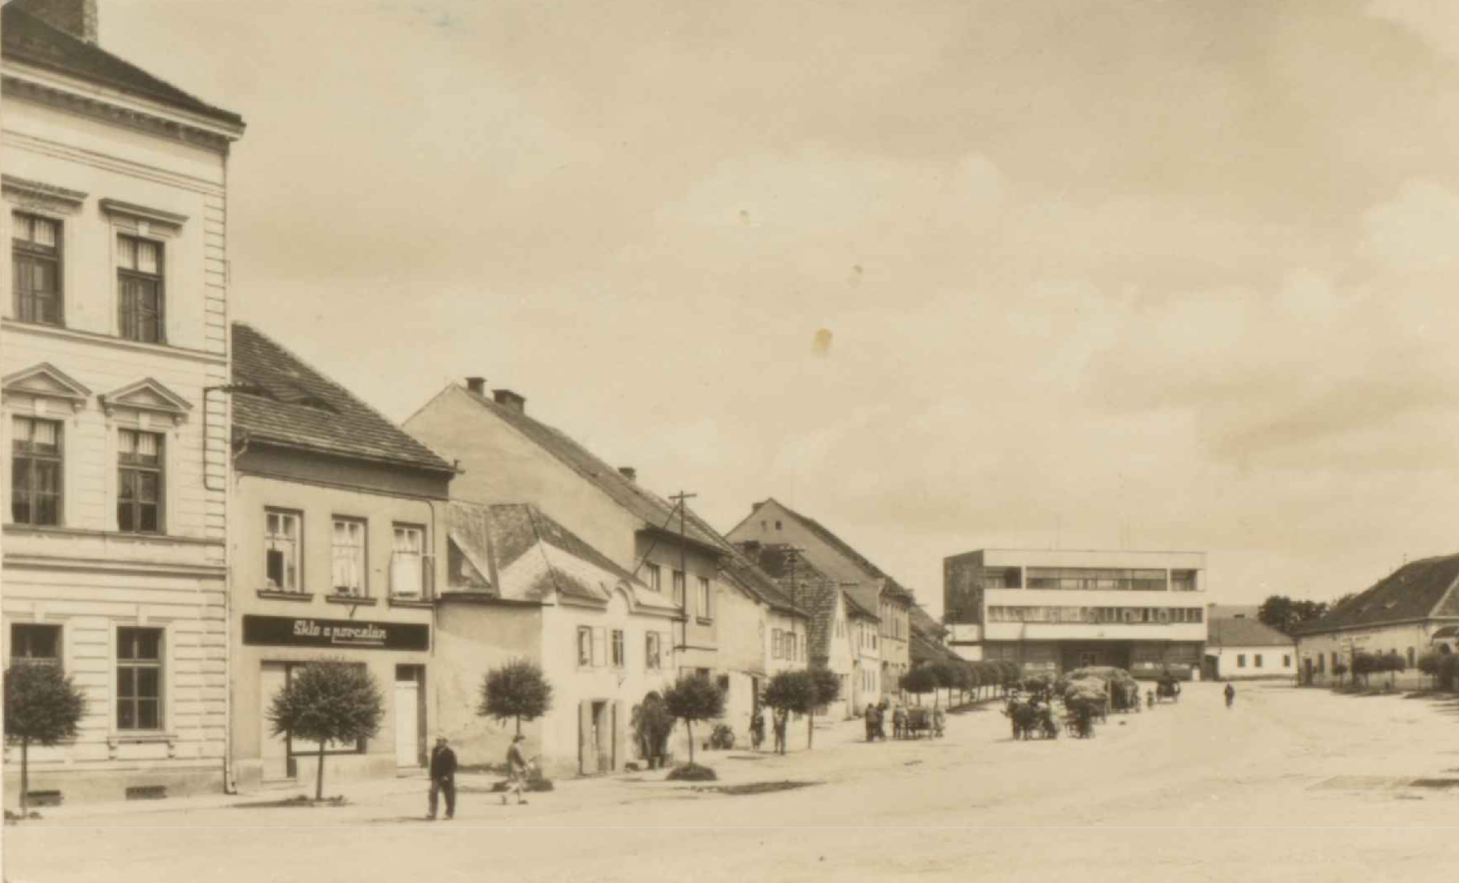
\includegraphics[width=\textwidth, height=\textheight, keepaspectratio]{150-a-kralovice}
\caption{Kralovice byly více než sto let okresním městem a žili zde a dosud žijí a pohřbeni jsou četní členové našeho rodu}
\label{fig:150-a-kralovice}
\end{figure}

\begin{figure}
\centering
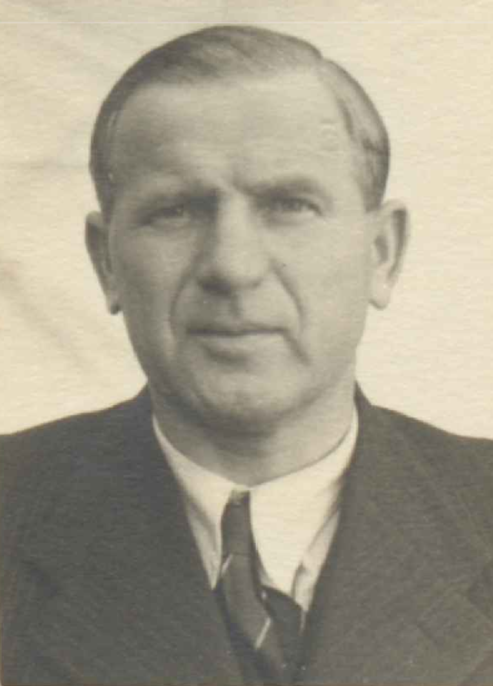
\includegraphics[width=\textwidth, height=\textheight, keepaspectratio]{150-b-josef_prusik_1893}
\caption{Josef Prusík, nar. 1893 v Chrašťovicích, bydlí v Kralovicích. Je dnes nejstarším žijícím Prusíkem v ČSR – nejmladším žijícím Prusíkem je Vladimír Prusík, narozený koncem května 1968 v Černotíně u Přeštic}
\label{fig:150-b-josef_prusik_1893}
\end{figure}

\begin{figure}
\centering
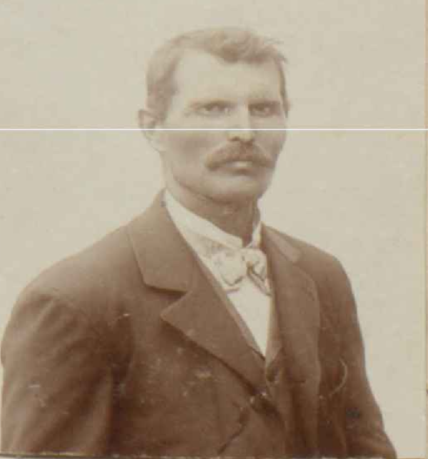
\includegraphics[width=\textwidth, height=\textheight, keepaspectratio]{150-c-vojtech_prusik_1856}
\caption{Vojtěch Prusík narozený 1856 ve Výrově u Kralovic byl zakladatelem agrární strany v tomto kraji. Byl dlouhá léta starostou ve Výrově a také úspěšným starostou okresu kralovického na počátku XX. století (1856 – 1920)}
\label{fig:150-c-vojtech_prusik_1856}
\end{figure}

% str 131-166 @ 151-156
% TODO seznam

\end{document}
